
	\chapter{Measuring Lamella Thickness and/or Lifetime via the Device}
		
	\section{Preparation}
	At first fill the glass chamber with \SI{25}{\milli\liter} of the sample solution. 
	Place the container on the stepper motor (see Fig. \ref{fig:chamberplacement}). 
	
	
	\begin{figure}
		\centering
		\begin{subfigure}[b]{0.4\textwidth}
			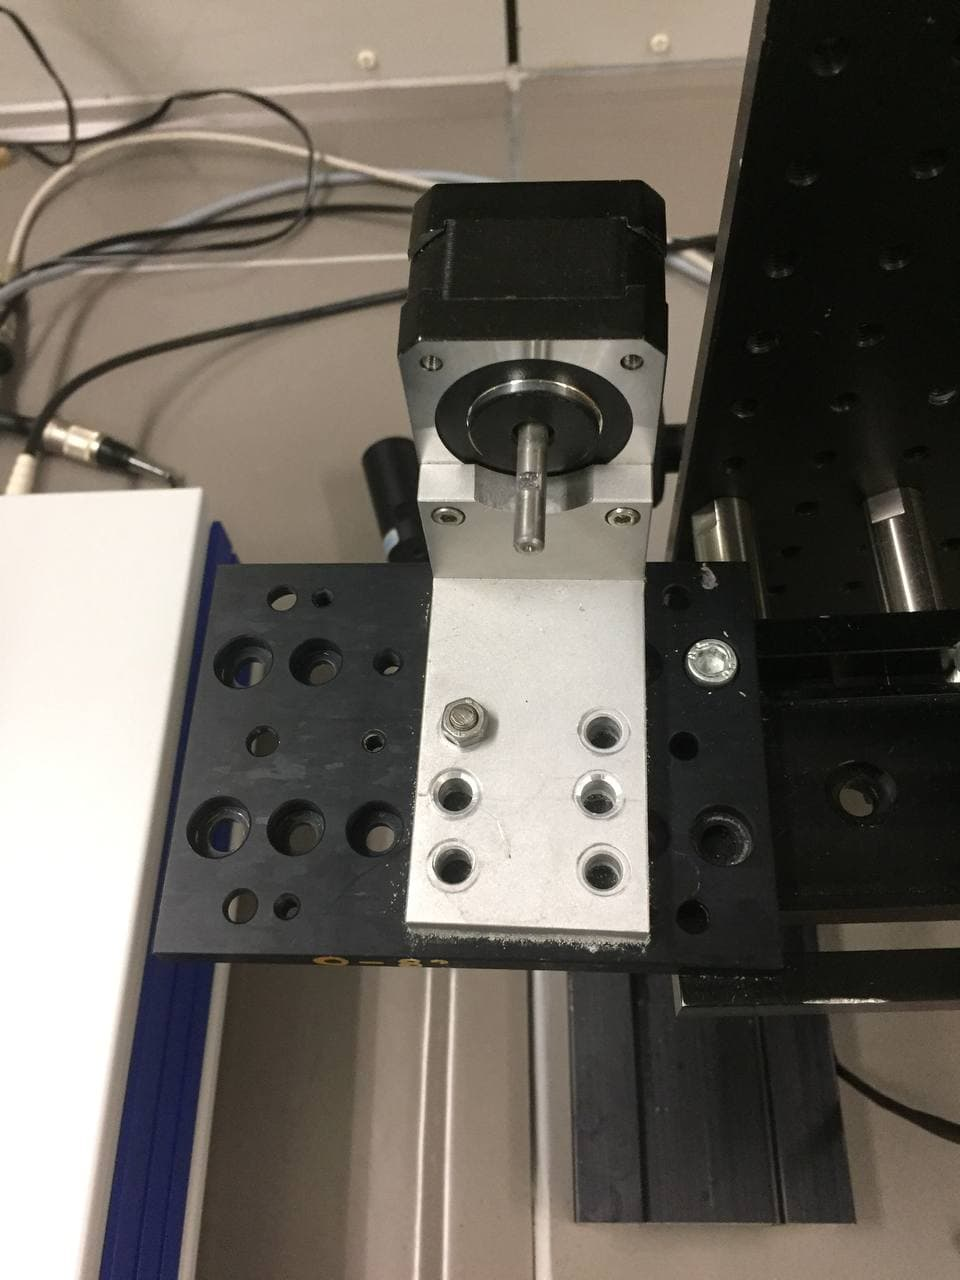
\includegraphics[width=\textwidth]{LamellaDevice_Hardware/PictureWithoutChamber}
			\caption{Stepper motor without chamber.}
		\end{subfigure} \hspace{0.1\textwidth}
		\begin{subfigure}[b]{0.4\textwidth}
			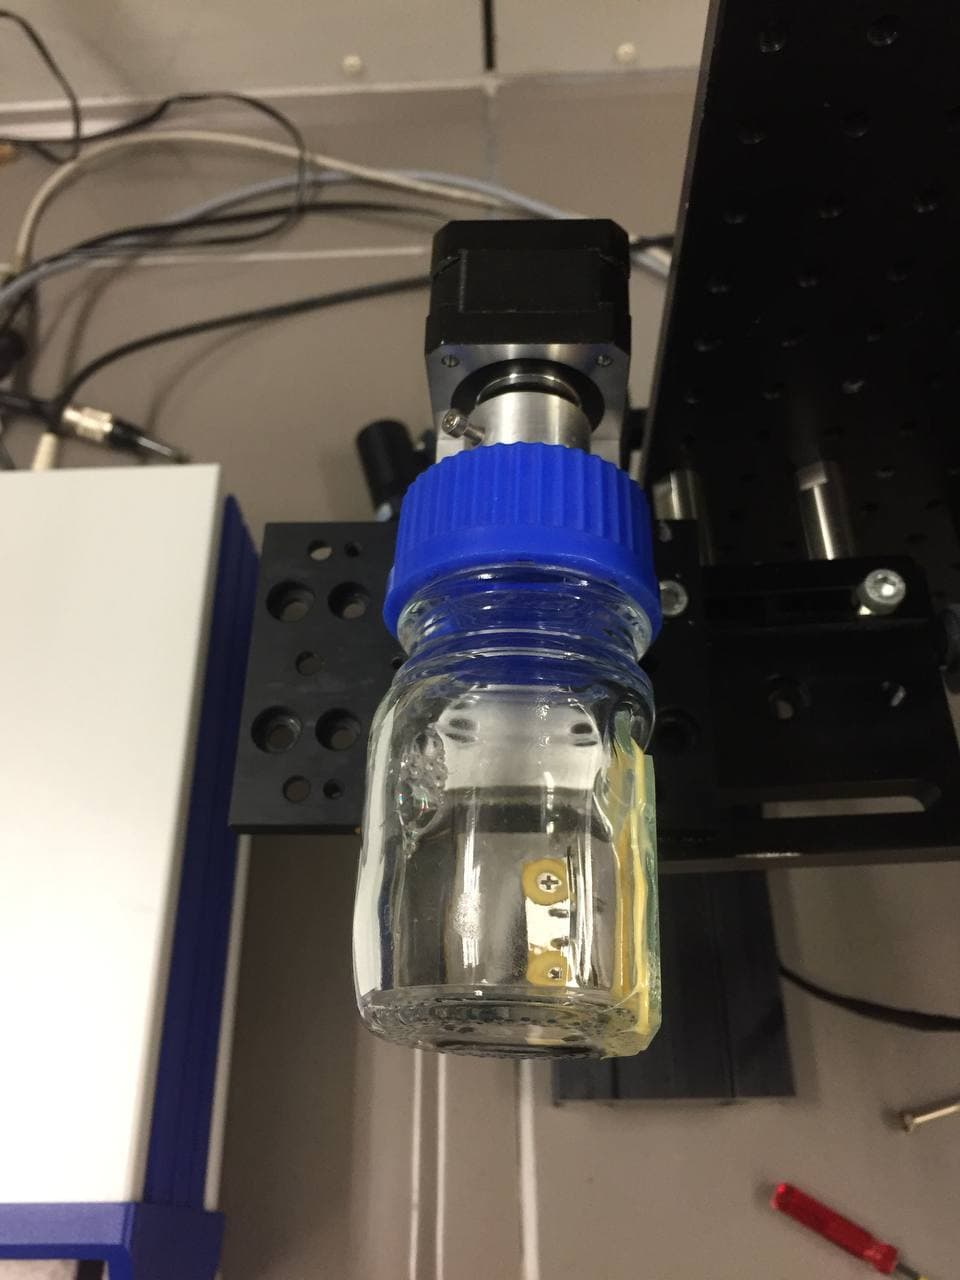
\includegraphics[width=\textwidth]{LamellaDevice_Hardware/PictureWithChamber}
			\caption{Stepper motor with chamber.\\}
		\end{subfigure}
	
		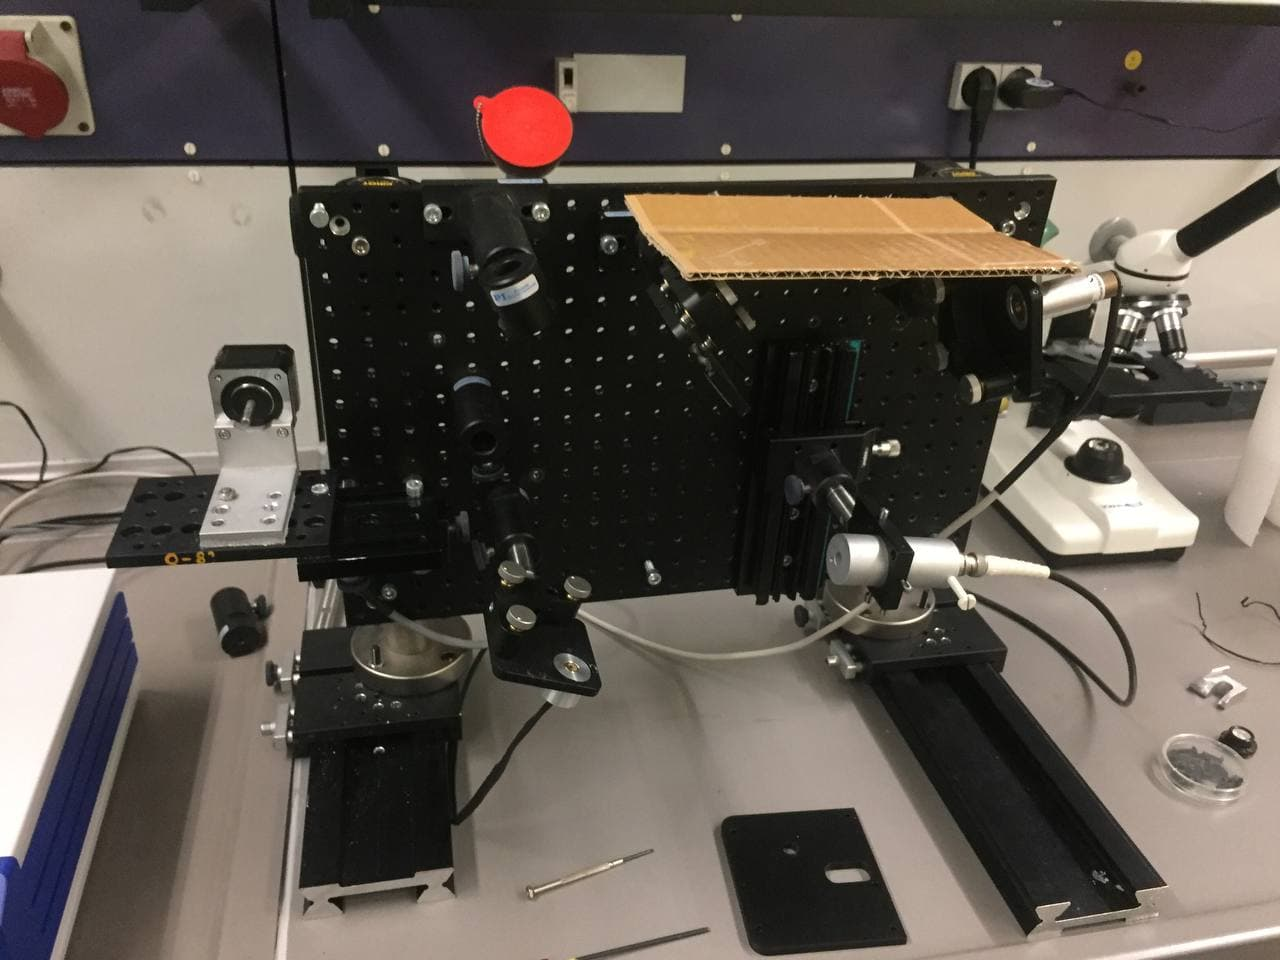
\includegraphics[width=0.9\textwidth]{LamellaDevice_Hardware/PictureOfApparatus}
		\caption{Photo of the apparatus}
		\label{fig:chamberplacement}
	\end{figure}
	
	\section{Measurement setup}
	Put the SD-Card into the slot and turn the device on. 

	You will be greeted by an error message, which can be ignored (Press on the backwards-arrow).
	Afterwards the home page will be started (Fig. \ref{fig:homepage}).
	
	Select what you want to measure. (This has only effects on the saved data.)
	
	On the next page (Fig. \ref{fig:parameterspage}), you can select the measurement parameters. 
	\textbf{Important: Turn at least 1 LASER on. }
	
	Short explanation of the parameters. 
	\begin{itemize}
		\item Number: How many lamellas should be measured
		\item Period: After which time should the lasers be changed? (in \SI{}{\milli\second})
		\item Max. Time: How long should one lamella be measured maximally? (in \SI{}{\minute})
	\end{itemize}
	
	By pressing "Additional Settings" a new page (Fig. \ref{fig:addsettingpage}) will open, which is not necessary for most measurements. 
	
	\begin{itemize}
		\item Formation: How long should the step motor stand in the formation position? (in \SI{}{\milli\second})
		\item Relaxation: How long should the lamella be ignored after formation? (in \SI{}{\milli\second})
		\item Confirmation: How long should the measurement value be under the threshold, before the lamella is detected as ruptured? (\SI{}{\milli\second})
		\item Threshold: At which detection value should the lamella be counted as ruptured? (in \SI{}{\milli\volt})
	\end{itemize}
	
	Confirm the settings with the button "!" and the next page will open (Fig. \ref{fig:setuppage}).
	
	\begin{figure}
		\centering
		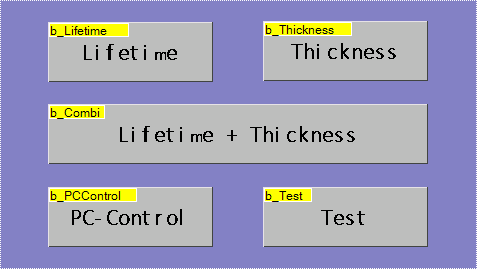
\includegraphics[width=0.7\linewidth]{LamellaDevice_Hardware/HomePage}
		\caption{Screenshot of the page ''Home''.}
		\label{fig:homepage}
	\end{figure}

	\begin{figure}
		\centering
		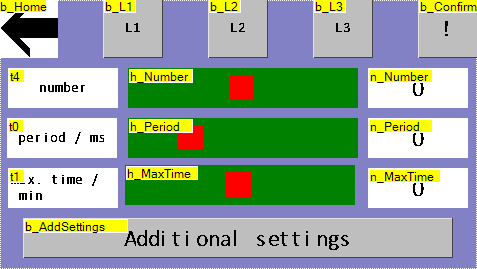
\includegraphics[width=0.7\linewidth]{LamellaDevice_Hardware/ParametersPage}
		\caption{Screenshot of the page ''Parameters''.}
		\label{fig:parameterspage}
	\end{figure}
	
	\begin{figure}
		\centering
		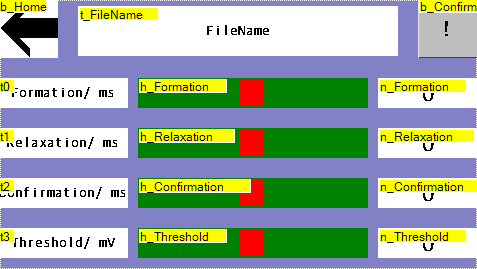
\includegraphics[width=0.7\linewidth]{LamellaDevice_Hardware/AddParametersPage}
		\caption{Screenshot of the page ''AddParameters''.}
		\label{fig:addsettingpage}
	\end{figure}

	\begin{figure}
		\centering
		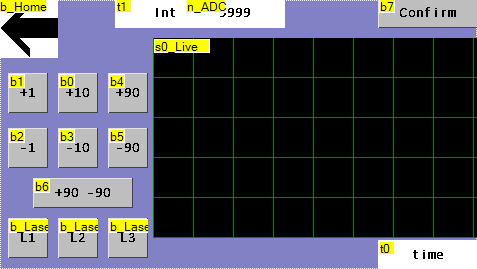
\includegraphics[width=0.7\linewidth]{LamellaDevice_Hardware/SetupPage}
		\caption{Screenshot of the page ''Setup''.}
		\label{fig:setuppage}
	\end{figure}
	
	\section{Orientate the chamber}
	After opening the setup page (Fig. \ref{fig:setuppage}) the measurement chamber needs to be orientated. For this following buttons are used:
	\begin{itemize}
		\item "+1"/"-1": One Step in clockwise ("+") or counter clockwise ("-") direction.
		\item "+10"/"-10": Ten steps in clockwise ("+") or counter clockwise ("-") direction.
		\item "+90"/"-90": 90 degrees in clockwise ("+") or counter clockwise ("-") direction.
		\item "+90 -90": Turn the chamber 90 degree in clockwise direction and after the formation time 90 degrees in counter clockwise direction.
		\item "L \textit{X}": Switch laser with number "x" on or off. 
	\end{itemize}
	
	In the diagram you can see the measured intensity. With two lasers turned on, it should be (shortly after formation) about 2 squares above the bottom and relatively constant. 
	
	By pressing confirm the measurement is started and the page shown in Fig. \ref{fig:measurementpage} is opened. 
	
	After finishing all measurements a "finished" message will be shown. The measurement can be stopped at every moment by pressing "Stop".
	
	
	\begin{figure}[h]
		\centering
		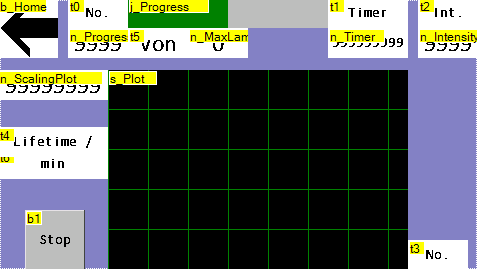
\includegraphics[width=0.7\linewidth]{LamellaDevice_Hardware/MeasurementPage}
		\caption{Measurement page}
		\label{fig:measurementpage}
	\end{figure}

	\section{Error Codes}
		\begin{tabular}{|c|c|}
			\hline 
			Code & Problem \\ 
			\hline 
			1 & Wrong Interrupt from Nextion Display received.\\
			\hline
			\hline
			100 & No laser is activated for measurement \\ 
			\hline 
			101 & No measurement mode is selected \\
			\hline
			\hline
			700 & File for lifetime logging could not be opened. \\ 
			\hline 
			701 & Write of lifetime to file failed.   \\ 
			\hline 
			702 & File for lifetime logging could not be closed. \\ 
			\hline 
			710 & File for speedtest logging could not be opened. \\ 
			\hline 
			711 & Write of speedtest data to file failed.   \\ 
			\hline 
			712 & File for speedtest logging could not be closed. \\ 
			\hline 		
			720 & File for intensity logging could not be opened. \\ 
			\hline 
			721 & Write of intensity value to file failed.   \\ 
			\hline 
			722 & File for intensity logging could not be closed. \\ 
			\hline 
		\end{tabular} 

	
	